%%%%%%%%%%%%%%%%%%%%%%%%%%%%%%%%%%%%%%%%%%%%%%%%%%%%%%%%%%%%%
% Matt Pitkin 26/04/05                                      %
%                                                           %
% Chapter 1: The Introduction - it starts ...               %
%%%%%%%%%%%%%%%%%%%%%%%%%%%%%%%%%%%%%%%%%%%%%%%%%%%%%%%%%%%%%

\chapquote{Well, the thing about a black hole - its main distinguishing feature - is it's black.
And the thing about space, your basic space colour is black. So how are you supposed to see
them?}{Holly - Red Dwarf}

\chapter{Introduction}

% blah blah blah
% gravitational wave this, gravitational wave that
This chapter will provide a brief overview of the theory behind gravitational radiation. A
selection of sources are discussed with emphasis on their potential to produce detectable
gravitational waves. A brief overview of the detection of \gws using interferometry is given.
Finally, a summary of a selection of previous searches for several types of \gw source is given.
% and some more

\section{The history and theory of gravitational radiation}
Prior to 1915 all conventional gravitational theory was Newtonian and in the equations of this
framework the force of gravity was thought of as any other force - the action of one body on
another - with, for the case of gravity, that action being instantaneous. Masses attracted other
masses because that was a property of mass. This theory provided no method for the production of
\gws which would only come about after a radical rethink of the theory of gravity\footnote{although
combining Newtonian gravity with special relativity, through the insertion of a delay, or
retardation, between the source, $\rho{}(x,t)$, and its Newtonian gravitational potential field,
$\phi(y,t-|x-y|/c)$, gives the basic properties from which \gws can be derived, as in Schutz (1984)
\cite{Schutz:1984}.}. With the publication of Einstein's General Theory of Relativity in 1915
\cite{Einstein:1915} gravity became a property of space-time itself (indeed the idea of space-time
as a combined entity $\{t,x,y,z\}$ in which the frame of reference was paramount had only just been
introduced), where mass/energy curved space-time and objects followed geodesics in this curved
manifold. From the equations of General Relativity (GR), as the theory is universally known, the
prediction of \gws - ripples in space-time - was quickly derived by Einstein \cite{Einstein:1918}.

\subsection{The basics of \gw theory}
This section will provide an overview of the derivation of \gws from GR, but is not meant to be an
in-depth description. A far fuller description can be found in Schutz (1985) \cite{Schutz:1985},
along with definitions of many of the terms and equations used herein.

GR describes the force of gravity in the new terms of geometry. This geometry is described by the
geodesic equation, which is the GR equivalent of the regular equation of motion $F = ma$, and the
Riemann curvature tensor (defined in \cite{Schutz:1985}).
%\begin{equation}
%R^{\alpha}_{\beta\mu\nu} \equiv \partial_{\mu}\Gamma^{\alpha}_{\beta\nu} -
%\partial_{\nu}\Gamma^{\alpha}_{\beta\mu} + \Gamma^{\alpha}_{\sigma\mu}\Gamma^{\sigma}_{\beta\nu} -
%\Gamma^{\alpha}_{\sigma\nu}\Gamma^{\sigma}_{\beta\nu}
%\end{equation}
The source of this curvature is the energy-momentum density and flux of space which is described by
the {\it stress-energy} tensor $T^{\alpha\beta}$. From these an equivalent of the Newtonian
gravitational potential field equation (or electromagnetic potential field), the general
relativistic field equation, known as Einstein's field equation, is defined (in natural units so
$G=c=1$) as,
\begin{equation}\label{EinsteinsFieldEqn}
G^{\alpha\beta} \equiv R^{\alpha\beta} - \frac{1}{2}g^{\alpha\beta}R = 8\pi{}T^{\alpha\beta},
\end{equation}
where $R^{\alpha\beta}$ and $R$ are the Ricci tensor and scalar describing the curvature of space
(from the Riemann tensor), and $g^{\alpha\beta}$ is the space-time metric describing transformations
relevant for the space-time. Deriving the formula for \gws comes straight from Einstein's field
equation in the weak field approximation. Under this approximation the metric $g_{\alpha\beta} =
\eta_{\alpha\beta} + h_{\alpha\beta}$, where $\eta_{\alpha\beta}$ is the Minkowski metric for flat
space ($\eta_{\alpha\beta~(\alpha=\beta)} = \{-1,1,1,1\}$ and $\eta_{\alpha\beta~(\alpha\ne \beta)}
 = 0$) and $h_{\alpha\beta}$ is some small perturbation with $|h_{\alpha\beta}| \ll 1$. The {\it
background Lorentz transforms}, again defined in \cite{Schutz:1985}, show that $h_{\alpha\beta}$
transforms as a tensor all by itself rather than just being part of $g_{\alpha\beta}$, so the
underlying space-time is always flat with $h_{\alpha\beta}$ defined on top of it. This allows us to
think of our curvature, and Riemann tensor, just in terms of $h_{\alpha\beta}$. For convenience the
metric perturbation $h_{\alpha\beta}$ is redefined as the {\it trace reverse}
\begin{equation}
\bar{h}^{\alpha\beta} = h_{\alpha\beta}- \frac{1}{2}\eta^{\alpha\beta}h.
\end{equation} 
Under the weak field approximation
equation~\ref{EinsteinsFieldEqn} reduces to
\begin{equation}\label{WeakFieldEqn}
\Box\bar{h}^{\alpha\beta} = -16\pi{}T^{\alpha\beta},
\end{equation}
which for the case of free space, where $T^{\alpha\beta} = 0$, becomes
\begin{equation}\label{WaveEqn}
\left(-\frac{\partial^2}{\partial{}t^2} + \nabla^2\right)\bar{h}^{\alpha\beta} = 0.
\end{equation}
It can be seen that equation~\ref{WaveEqn} is the three-dimensional wave equation, the solution of
which for the simplest plane waves is
\begin{equation}
\bar{h}^{\alpha\beta} = A^{\alpha\beta}\exp{(ik_{\alpha}x^{\alpha})},
\end{equation}
showing that small perturbations in space-time will propagate as a wave. Through further proofs, as
given in \cite{Schutz:1985}, it can be shown that this wave will propagate at the speed of light.
Applying the {\it transverse-traceless} gauge conditions Schutz \cite{Schutz:1985} shows that the
wave will be transverse and that the tensor has the form
\begin{equation}
h_{\alpha\beta}^{\rm TT} = \left( \begin{array}{cccc}
0 & 0 & 0 & 0 \\
0 & \bar{h}_{xx} & \bar{h}_{xy} & 0 \\
0 & \bar{h}_{xy} & -\bar{h}_{xx} & 0 \\
0 & 0 & 0 & 0
\end{array} \right),
\end{equation}
i.e. if the wave is travelling in the $z$ direction it will only have amplitude components in the
$x$ and $y$ directions, and with only two independent amplitude values $A_{xx}^{\rm TT}$ and
$A_{xy}^{\rm TT}$. The fact that the tensor must be traceless, $A^{\alpha}_{~\alpha}=0$, implies
that $\bar{h}_{\alpha\beta}^{\rm TT} = h_{\alpha\beta}^{\rm TT}$.

In a coordinate dependent system the effect of a \gw will not be seen. However, we can see how these
waves (metric perturbations) affect particles by looking at their effect on the proper distance
$d\ell$ between two such particles. Applying the equation of geodesic deviation it can be shown,
again in Schutz (1985) \cite{Schutz:1985}, that for two particles separated in the $x$-direction,
with 4-velocity $\vec{U} = (1,0,0,0)$ and separation vector $\vec{\xi} = (0,\epsilon,0,0)$, that
\begin{equation}\label{gwmotion}
\frac{\partial^2}{\partial{}t^2}\xi^x = \frac{1}{2}\epsilon\frac{\partial^2}{\partial{}t^2}
h_{xx}^{\rm TT},~{\rm and}~
\frac{\partial^2}{\partial{}t^2}\xi^y = \frac{1}{2}\epsilon\frac{\partial^2}{\partial{}t^2}
h_{xy}^{\rm TT}.
\end{equation}
Considering two particles initially having a separation vector $\vec{\xi} =
(0,\epsilon\cos{\theta}, \epsilon\sin{\theta}, 0)$, we get acceleration in $\xi$ of
\begin{equation}\label{geodev1}
\frac{\partial^2}{\partial{}t^2}\xi^x = \frac{1}{2} \epsilon \cos{\theta}
\frac{\partial^2}{\partial{}t^2} h_{xx}^{\rm TT} + \frac{1}{2} \epsilon \sin{\theta}
\frac{\partial^2}{\partial{}t^2} h_{xy}^{\rm TT},
\end{equation}
and
\begin{equation}\label{geodev2}
\frac{\partial^2}{\partial{}t^2}\xi^y = \frac{1}{2} \epsilon \cos{\theta}
\frac{\partial^2}{\partial{}t^2} h_{xy}^{\rm TT} - \frac{1}{2} \epsilon \sin{\theta}
\frac{\partial^2}{\partial{}t^2} h_{xx}^{\rm TT}.
\end{equation}
Using the real part of the plane wave solution to the wave equation (with us stationary at $z=0$),
so $h_{\alpha\beta}^{\rm TT} = A_{\alpha\beta}\cos{(\omega{}t)}$, as shown by Hendry
\cite{Hendry:2005}, gives
solutions to equations~\ref{geodev1} and \ref{geodev2} in $x$ and $y$ of
\begin{equation}\label{gwmotionx}
\xi^x = \epsilon\cos{\theta} + \frac{1}{2}\epsilon\cos{\theta}A_{xx}^{\rm TT}\cos{\omega{}t} +
\frac{1}{2}\epsilon\sin{\theta}A_{xy}^{\rm TT}\cos{\omega{}t},
\end{equation}
and
\begin{equation}\label{gwmotiony}
\xi^y = \epsilon\cos{\theta} + \frac{1}{2}\epsilon\cos{\theta}A_{xy}^{\rm TT}\cos{\omega{}t} -
\frac{1}{2}\epsilon\sin{\theta}A_{xx}^{\rm TT}\cos{\omega{}t}.
\end{equation}
If we have a ring of particles at various angles between 0 and $2\pi$ radians these equations
show how the passing of a plane \gw effects them in terms of the proper distance between them and
the centre of the ring (see fig~\ref{ringofparticles}). These equations show that because of the
independence of $h_{xx}^{\rm TT}$ and $h_{xy}^{\rm TT}$ we have two distinct linear polarisations of
the wave, one when $h_{xx}^{\rm TT} \ne 0$ and $h_{xy}^{\rm TT}=0$ and the other when $h_{xx}^{\rm
TT} = 0$ and $h_{xy}^{\rm TT}\ne0$. These two states, called `plus' (+) and `cross' ($\times$) are
seen in figure~\ref{ringofparticles} to be rotated by $45^{\circ}$ to each other, as opposed to
electromagnetic wave polarisation states with a rotation of $90^{\circ}$.
\begin{figure}[!htbp]
\begin{center}
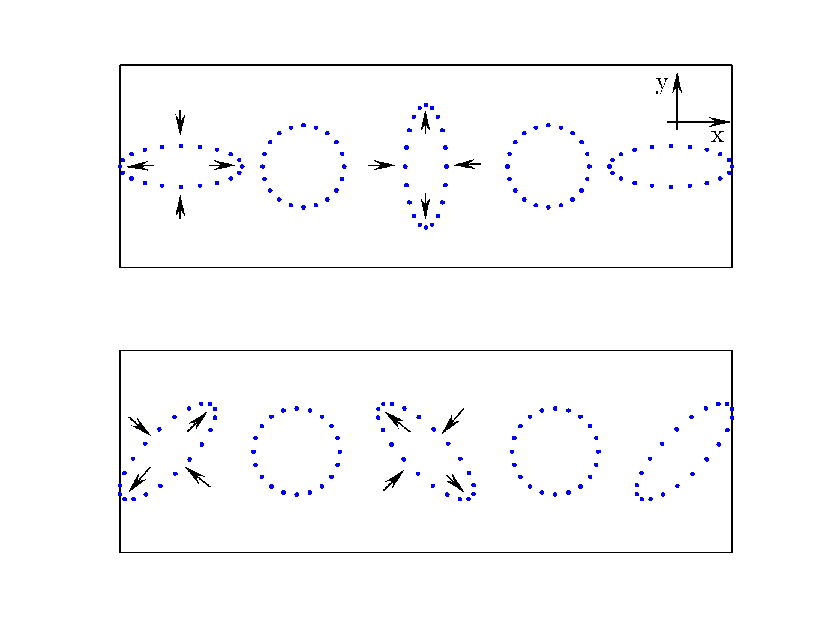
\includegraphics[width=0.6\textwidth]{figs/ringofparticles}\caption[Effect of a \gw on a ring of
particles.]{The effect of a plane \gw on a ring of particles over one wavelength for the +
polarisation (top) and the $\times$ polarisation (bottom).}\label{ringofparticles}
\end{center}
\end{figure}

\subsection{Generation of gravitational waves}
The equations above described how a \gw propagates through space, but says nothing about their
generation as the {\it stress-energy} tensor is set to zero. To study the generation of \gws we
will have return to equation~\ref{WeakFieldEqn} and follow the methodology shown in Schutz (1985)
\cite{Schutz:1985}. The solutions of this are simplified through two assumptions: i) the time
dependent part of $T_{\alpha\beta}$ is sinusoidal with angular frequency $\Omega$; and ii) the
source is small compared to the wavelength of radiation emitted, $\epsilon \ll 2\pi/\Omega$.
Under these assumptions the solution for $\bar{h}_{\alpha\beta}$, to lowest order, has the form
\begin{equation}
\bar{h}_{\alpha\beta} = 4J_{\alpha\beta}e^{i\Omega(r-t)}/r,
\end{equation}
where $r$ is the distance from the source. The $J_{\alpha\beta}$ term can be written in the form of
the quadrupole moment of the mass distribution
\begin{equation}\label{QuadMomDefEqn}
I^{lm} \equiv \int T^{00}x^lx^m{\rm d}^3x \approx \int \rho x^lx^m{\rm d}^3x,
\end{equation}
where $T_{00} \approx \rho$ is the mass density (under the assumption that the source motion is
slow i.e. $v \ll c$), so
\begin{equation}
J_{\alpha\beta}e^{-i\Omega{}t} = \frac{1}{2}\frac{{\rm d}^2}{{\rm d}t^2}I_{\alpha\beta}.
\end{equation}
From this we can write our solution as
\begin{equation}\label{QuadMomEqn}
\bar{h}_{jk} = -2\ddot{I}_{jk}/r = -2\Omega^2I_{jk}e^{i\Omega{}r}/r.
\end{equation}
It can be shown, as in Flanagan and Hughes (2005) \cite{Flanagan:2005}, that the lower order moments
of the mass distribution (zeroth and dipole) are ruled out as contributing to the \gw emission
through the conservation of mass/energy and angular momentum respectively. A simple approximation of
the quadrupole moment for a source with total mass $M$ and size $R$, shows that $I_{jk}$ is of order
$MR^2$. Equation~\ref{QuadMomEqn} can be used to get a simple estimate of the \gw amplitude (as
shown in Schutz, 1999 \cite{Schutz:1999}) by noting that for non-spherical motions the components
of $\ddot{I}_{jk}$ will have magnitudes or order $Mv^2$, where $v$ is the non-spherical component
of the velocity inside the source. Given this an approximate amplitude will be
\begin{equation}\label{SimpleQuadMomEqn}
h \sim 2Mv^2/r
\end{equation}
(or $h \sim 2GMv^2/c^4r$ converting back to SI units). It should be stated that spherically
symmetric motions will not radiate.

Again we can make a gauge restriction and find a {\it transverse-traceless} gauge which gives the
simplest form of the wave. In such a gauge the quadrupole moment becomes the reduced quadrupole
moment tensor,
\begin{equation}
I_{jk} \to I_{jk} - \frac{1}{3}\delta_{jk}I^l_{~l}.
\end{equation}
With axis aligned so that the wave is travelling in the $z$-direction we get components of our
perturbation given by
\begin{eqnarray}
\bar{h}^{\rm TT}_{zi} & = & 0, \\
\bar{h}^{\rm TT}_{xx} & = & -\bar{h}^{\rm TT}_{yy} = -\Omega^2(I_{xx} - I_{yy})e^{i\Omega{}r}/r, \\
\bar{h}^{\rm TT}_{xy} & = & -2\Omega^2I_{xy}e^{i\Omega{}r}/r.
\end{eqnarray}
These show that the reduced quadrupole moment provides the main factor in the \gw amplitude. This
method is not the exact solution but is in general a good approximation for simple sources and for
providing estimates of source strength.

We will consider the example of two stars in a binary system separated by $R$ and of equal mass
$m$ (as shown in \cite{Flanagan:2005}). If we chose these to be lying in the $x-y$ plane, then in
our coordinates $x = x_1 = R\cos{\Omega{}t}$, $y = x_2 = R\sin{\Omega{}t}$ and $z = x_3 = 0$. The
reduced quadrupole moment for this system is
\begin{eqnarray}
I_{jk} & = & \mu\left(x_jx_k - \frac{1}{3}\delta_{jk}r^2\right) \\
 & = & \mu{}R^2\left( \begin{array}{ccc}
 {\rm cos}^2\Omega{}t - \frac{1}{3} & \cos{\Omega{}t}\sin{\Omega{}t} & 0 \\
 \cos{\Omega{}t}\sin{\Omega{}t} & {\rm cos}^2\Omega{}t - \frac{1}{3} & 0 \\
 0 & 0 & -\frac{1}{3} \end{array}\right)
\end{eqnarray}
where $\mu = m_1m_2/(m_1 + m_2) = m/2$ is the reduced mass of the system, giving coefficients of the
time varying parts of the second derivative, $\ddot{I}_{jk}$, as $-2\Omega^2\mu{}R^2$. This gives a
typical magnitude for $h$ of
\begin{equation}
h \approx \frac{4\mu\Omega^2R^2}{r}.
\end{equation}
In this example we can use Kepler's third law ($R^3\Omega^2 = GM$, where $M = 2m$ is the total mass)
to give (in SI units)
\begin{equation}\label{binaryamp}
h = \frac{(GM)^{5/3}\Omega^{2/3}}{c^4r}.
\end{equation}
Values will be placed on this for realistic examples in \S\ref{GWsources}. For two unequal masses
$M (=m_1+m_2)$ will be replaced by the {\it chirp mass} $\mathcal{M} = \mu^{3/5}M^{2/5}$. These \gws
will be have a completely circular polarisation perpendicular to the plane and completely linear
polarisation along the plane.

The frequency of \gws can often, as with the above example, be related to motions of the source,
but in many cases it is also related to the natural frequency of a self-gravitating body 
\begin{equation}\label{naturalfreq}
f = \sqrt{G\bar{\rho}/4\pi} \approx (1/2\pi)\sqrt{GM/R^3},
\end{equation}
where $\bar{\rho}$ is the mean mass-energy density \cite{Schutz:1999}. Some examples of this will be
given in \S\ref{GWsources}.

The energy carried away by \gws (the source's luminosity) is given by
\begin{equation}\label{gwluminosity}
\frac{{\rm d}E}{{\rm d}t} = L = -\frac{G}{5c^5}\langle \dddot{I}_{jk}\dddot{I}^{jk}\rangle.
\end{equation}
This can be useful for estimating the timescale over which objects will emit gravitational waves.

\section{Sources of gravitational waves}\label{GWsources}
The above equations can be used to derive the approximate strength of \gws for simplified sources.
From these we can estimate what kind of systems will yield detectable levels of radiation. Some
sources and their classification are discussed below, with more thorough reviews to be found in
Thorne (1987) \cite{300Years} and Schutz (1999) \cite{Schutz:1999}. 

\subsection{Man-made sources}
We could consider the possibility making some sort of \gw generator on human scales and then
estimating the level of radiation. Following the example in \cite{Schutz:1999} we will construct
something analogous to the binary star system described above, consisting of two $10^3$\,kg masses
held 10\,m apart by a light rigid beam rotating about its centre at a frequency of 10\,Hz. As all
the motion is non-spherical we will approximate $h$ using equation~\ref{SimpleQuadMomEqn}, with
velocity $v \sim 300\,{\rm m}{\rm s}^{-1}$. The distance to the source $r$ must be at least one
wavelength away in order to detect the \gws rather than the nearby Newtonian field. For our
generator the emission will be at twice the rotation frequency $f = 20$\,Hz as the mass distribution
is symmetric about the rotation axis, and the corresponding wavelength will be $\lambda =
1.5\ee{7}$\,m. So given these values we get an estimate of the \gw amplitude $h \sim 1\ee{-43}$,
which is $\sim 20$ orders of magnitude below the level we can expect to be able to detect. This
shows that human scale objects are not good sources, so we need to look elsewhere for possible
sources. In the universe, however, there are many environments with extreme energetics where the
mass-energy densities are at levels which begin to look more plausible as detectable \gw generators.
These will now be discussed.

\subsection{Continuous wave sources}
A continuous (or periodic) wave source is one that emits a quasi-sinusoidal signal over a long
period. This feature will allow any detection strategy to build up signal-to-noise over a long
period of observation. The fact that the signal is persistent means that the source must not be
strongly damped (via \gw or electromagnetic emission, particle acceleration or other mechanisms),
or must have some source of power. The most obvious choice of sources with these properties are
those with intrinsic frequencies due to their own orbital or rotational motion.

\subsubsection{Neutron stars}
Neutron stars are discussed in more detail in Chapter~2, but here we will described the basics of
their continuous wave emission mechanism. Neutron stars (seen as pulsars or inferred in High and Low
Mass X-ray Binaries - LMXBs) are known to spin with precise frequencies and small spin-down rates,
i.e. they are damped slowly, therefore fulfilling both the criteria above for a continuous wave
source. Due to their extremely high gravitational field neutron stars are thought to be close to
spherical, but to generate \gws there must be some form of asymmetry about the rotational axis.
The two main forms of rotational asymmetry will be if the star is triaxial (oblate or prolate) or
precessing (rotation of the spin axis). If we consider the case of a triaxial star with a bump or
mountain (of mass $m$) giving our non-sphericity, then we can estimate the \gw amplitude via
equation~\ref{SimpleQuadMomEqn} as in \cite{Schutz:1999}. Given a radius $R$ and rotational
frequency $\nu$ (emission will be at $2\nu$ as rotation is about the centre of mass) we get $h \sim
16\pi^2GmR^2\nu^2/c^4r$. It can be seen that for this case the quadrupole moment is $mR^2 =
\varepsilon{}I_{zz}$, where $\varepsilon = (I_{xx}-I_{yy})/I_{zz}$ is the star's equatorial
ellipticity, and $I_{zz}$ is the principal moment of inertia about the rotation axis. We can write
this using some canonical neutron star values giving
\begin{equation}
h \approx 4.2\ee{-26}\left(\frac{I_{zz}}{10^{38}{\rm
kg\,m}^2}\right)\left(\frac{\varepsilon}{10^{-6}}\right)\left(\frac{\nu}{100\,{\rm
Hz}}\right)^2\left(\frac{1\,{\rm kpc}}{r}\right),
\end{equation}
where the value of $\varepsilon$ is on the upper end of plausible values for conventional neutron
star equations of state. This shows that in general this mechanism produces quite weak
gravitational waves, although the abundance of neutron stars and the fact that signal-to-noise can
be built up over time means they are a good potential source within our galaxy. It can be seen in
figure~\ref{designcurves1year} that for one year of observations with the LIGO detectors at design
sensitivity we are reaching into this range, and for Advanced LIGO (AdvLIGO) we should be in a range
with many potential sources.
\begin{figure}[!htbp]
\begin{center}
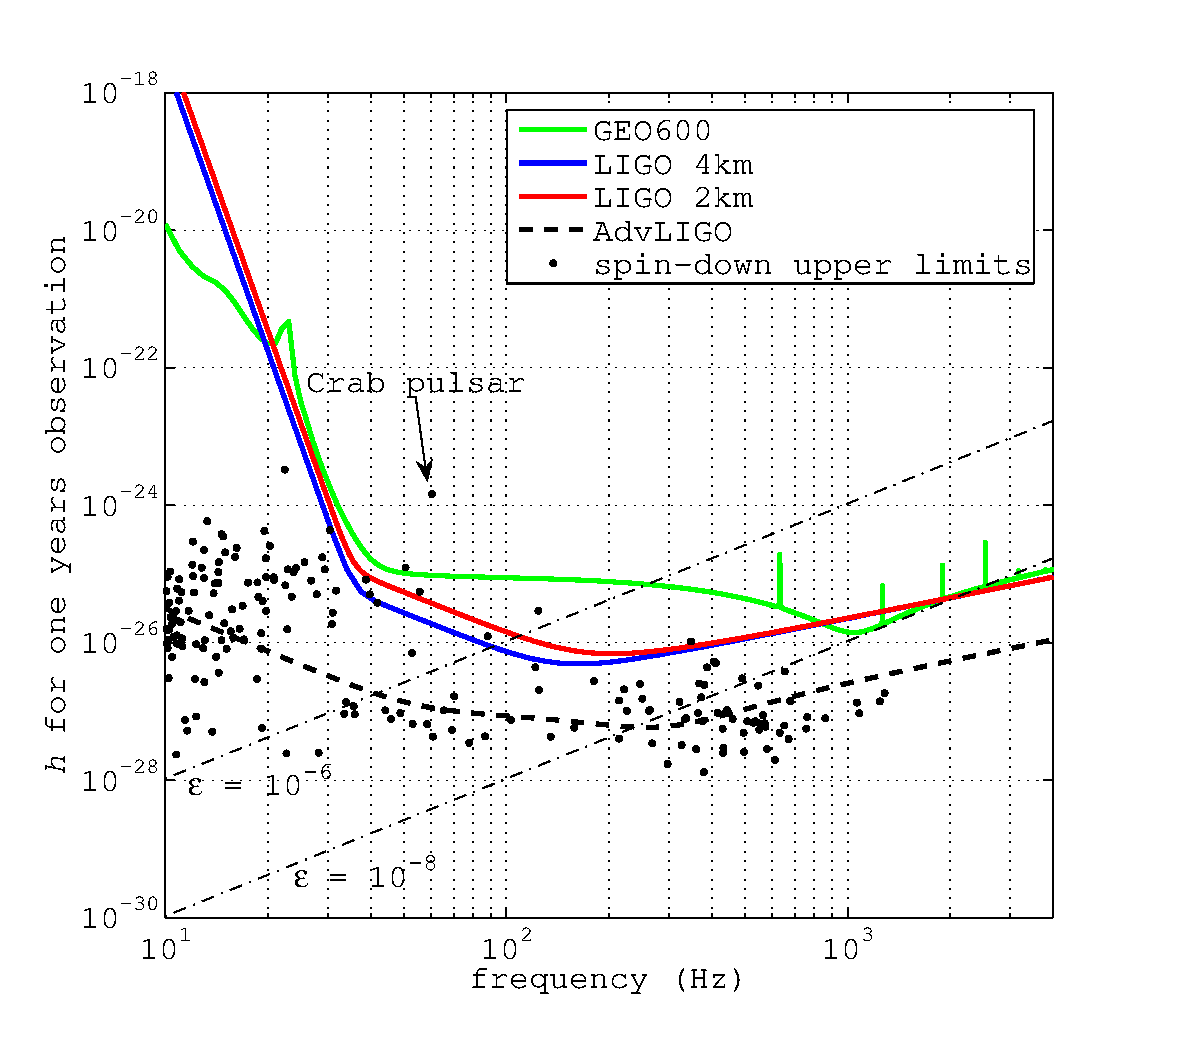
\includegraphics[width=0.6\textwidth]{figs/designcurves1year}\caption[The sensitivity
of the G\textsc{eo}\,600, LIGO and Advanced LIGO detectors for one year of observations.]{The
sensitivity of the \geo (tuned to 1000\,Hz), LIGO and Advanced LIGO detectors for one year of
observations. The Advanced LIGO design sensitivity is the current best estimate and subject to small
changes. Included are lines representing the expected \gw amplitude from a pulsar with an equatorial
ellipticity $\varepsilon$ of $10^{-6}$ and $10^{-8}$ at a distance of 1\,kpc, with $I_{zz} =
10^{38}$\,kg\,${\rm m}^2$. The spin-down upper limits (equation~\ref{spindownUL}) for all known
pulsars with $\nu > 5$\,Hz are also plotted.}\label{designcurves1year}
\end{center}
\end{figure}

Free precession of a neutron star requires some mechanism to sustain it and is generally strongly
damped. With only one pulsar (PSR\,B1828-11) known to exhibit free precession, and a few more
decreasingly likely candidates \cite{Culter:2003}, the population of sources is also likely
to be small. It therefore provides a far less likely source of gravitational waves, with the
calculations of Jones and Andersson (2002) \cite{JonesAndersson:2002} giving amplitudes of
\begin{equation}
h_0 \sim 10^{-27}\left(\frac{\Omega_w}{0.1}\right)\left(\frac{1\,{\rm 
kpc}}{r}\right)\left(\frac{f_s}{500\,{\rm Hz}}\right)^2,
\end{equation}
where $\Omega_w$ is the wobble angle, and $f_s$ is the signal frequency, which is well below the 
level of sensitivity of LIGO, but may be a source for AdvLIGO.

Hot, newly formed neutron stars, or stars heated up during accretion from a companion, could provide
continuous \gws due to emission from hydrodynamic waves on the surface or within the star. Such a
type of wave is the r-mode \cite{Andersson:1998}, which is driven by the rotation of the star and is
analogous to Rossby (or planetary) waves on the Earth driven by the Coriolis force. For newly formed
stars this could provide continuous wave emission for maybe up to a year after formation, until the
star has cooled and spun-down sufficiently \cite{Schutz:1999}. For accreting stars, i.e. in LMXBs,
the accretion can spin-up the star's rotation such that \gw emission could provide a natural
frequency limit at which \gw energy loss balances that spinning-up the star. As such the \gw
emission would be directly related to the systems X-ray luminosity.

\subsubsection{Binary systems} 
The other main source of continuous waves will be binary or multiple systems. All orbiting systems
will emit \gws to some extent (as in our man-made generator example), but the scale of the system
will be important in whether the waves are detectable. Evidence for the existence of \gws was in
fact inferred by the study of a neutron star binary system discovered by Hulse and Talyor (1975)
\cite{HulseTaylor:1975, TaylorWeisberg:1989} in which the orbit was losing energy exactly as
expected if carried away by gravitational radiation. As seen above \gws will be emitted at twice the
frequency of the orbital motion, with the amplitude proportional to the frequency squared and the
masses involved. Through the emission of gravitational radiation binaries will eventually inspiral,
increasing in frequency and therefore amplitude until coalescence. As an example of this we can find
the \gw amplitudes and coalescence times for a variety of systems. We will start with the nearest
stellar system to our own, the $\alpha$ and $\beta$-Centauri system. This system lies at a distance
of 4.35\,ly with two stars of roughly $1\,{\rm M}_{\odot}$ having an orbital period of 80 years ($f
= 4\ee{-10}$\,Hz) and a separation of 23\,AU. Using equation~\ref{binaryamp} we can calculate the
amplitude of \gws seen at Earth as $h \sim 6\ee{-23}$, which would be large enough for detection
were it at much higher frequencies, but is well out of the frequency range of any planned detector
(see figure~\ref{noisespectrumall}). The {\it chirp time} (or time to coalescence) of the binary can
also be estimated by making use of its luminosity and current kinetic energy ($ = -1/2$\,potential
energy $= Gm_1m_2/2R = G\mu{}M/2R$) via $t_{\rm chirp} = 1/4(E_{\rm binary}/L_{\rm binary}) \sim
10^{23}$\,years (from a luminosity of $L_{\rm binary} \sim 10^6$\,W). This shows that for main
sequence binary systems the \gw emission will take many orders of magnitude longer than the Hubble
time to cause noticeable orbital decay.

To get to amplitude levels and frequencies necessary for observations the binary systems must be
much more compact, therefore with much faster periods, and/or have much more massive components,
like supermassive black holes. For many systems made up of stellar remnants i.e. white-dwarfs,
neutron stars or stellar mass black holes, orbital periods on the order of hours are seen. Such
systems will also have chirp times within the age of the universe, leading to the possibility of
observing the final inspiral (discussed below). There are predicted to be many galactic double
white-dwarf binary systems $\sim 10^8$ (see Nelemans {\it et al.}, 2001 \cite{Nelemans:2001}), a
proportion of which with orbital periods of a few hours (some of which have been observed, Saffer
{\it et al.}, 1998 \cite{Saffer:1998}). These provide a large population of sources around $f \sim
10^{-4}$\,Hz, with \gw amplitudes (assuming two $0.5\,{\rm M}_{\odot}$ white-dwarfs and a distance
of 100\,light years) of $h \sim 10^{-21}$. Again as these are continuous sources, the
signal-to-noise can be built up over time. Due to the large amount of sources there could be much
source confusion with a noise floor made up of overlapping binary systems (see
figure~\ref{noisespectrumall}). This presents a potential challenge for LISA\footnote{LISA is a
future spaced-based interferometric \gw detector designed to view the low frequency band from $\sim
10^{-4} - 10^{-1}$\,Hz, and will be discussed briefly later.} data analysis in this frequency range.

As well as double white-dwarf systems, there are currently five {\it known} galactic double neutron
star systems (see Burgay {\it et al.}, 2003 \cite{Burgay:2003}), although the total population of
these will be far smaller than for white-dwarfs. These all have period of a few hours leading to an
estimate for the amplitude at a similar level to that for the white dwarfs. The population of
galactic black hole binaries will also be quite small and again produce \gws of a similar order of
magnitude.

Black hole binaries consisting of supermassive black holes, for example those found at the centre
of most galaxies, start to become of interest on cosmological distance scales. Such systems of
black holes with $M \gtrsim 10^6\,{\rm M}_{\odot}$ are likely to be visible to LISA throughout the
entire universe with amplitudes as shown in figure~\ref{noisespectrumall}.
\begin{figure}[!htbp]
\begin{center}
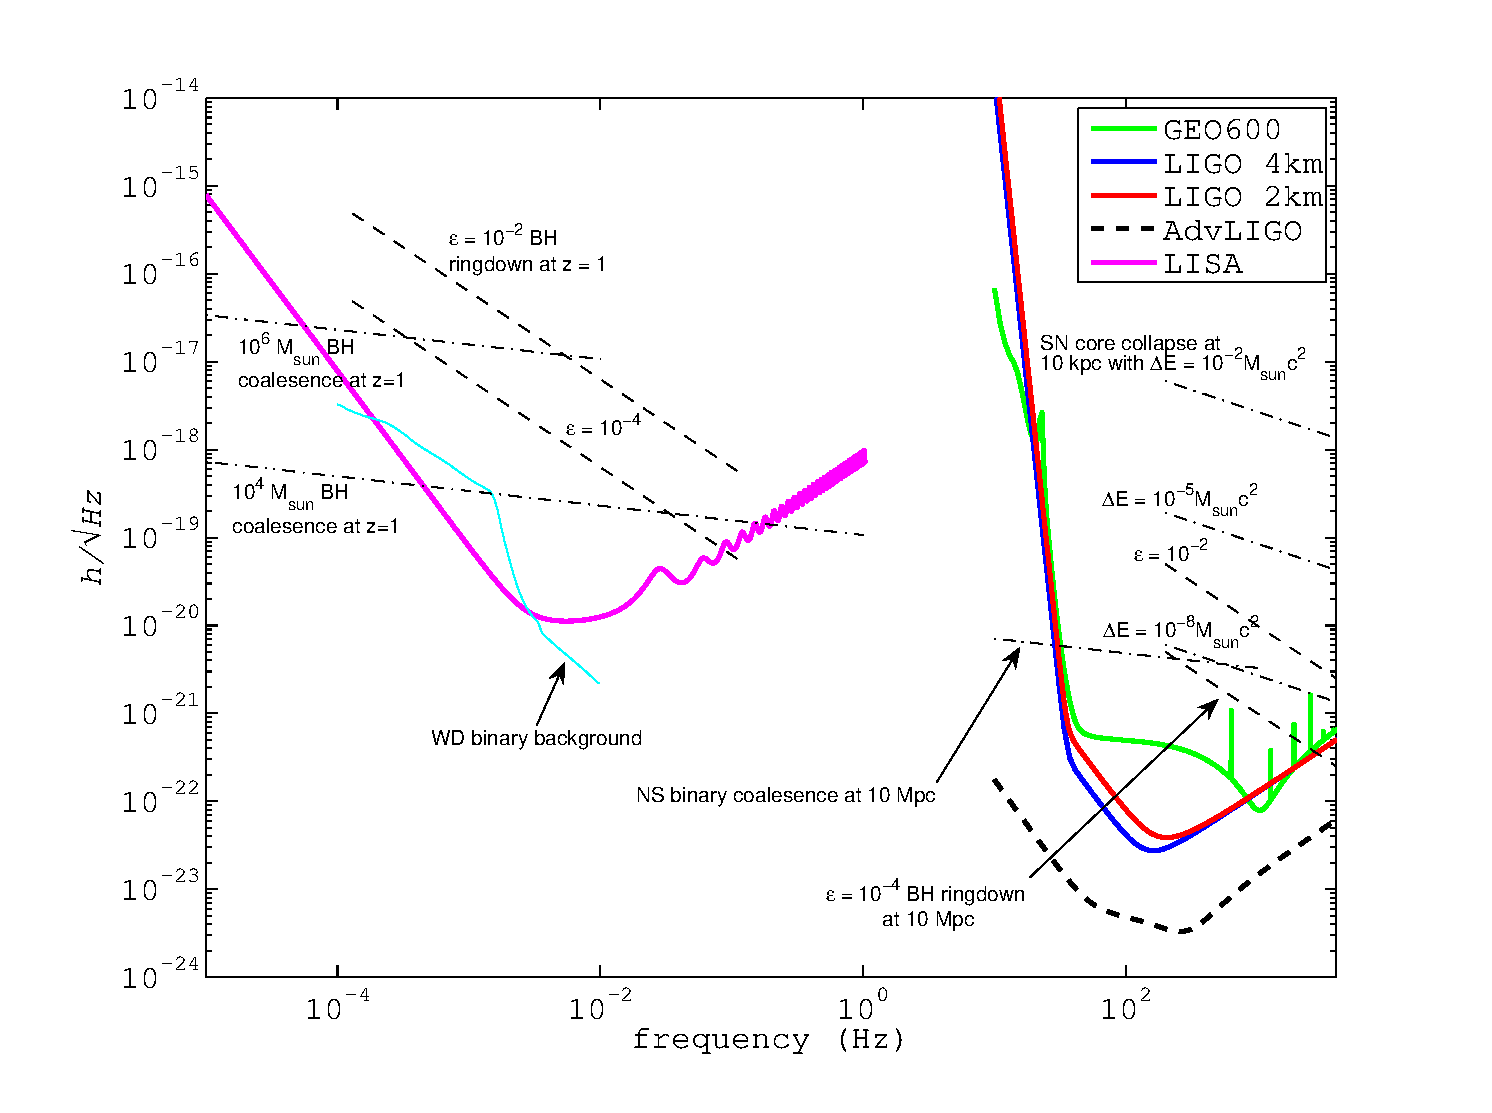
\includegraphics[width=0.8\textwidth]{figs/noisespectrumall}\caption[Detector noise curves and
source amplitudes.]{The noise spectrum of the current ground based interferometers (\geo and the
LIGO detectors), the proposed Advanced LIGO upgrade and the planned space-based detector LISA. Also
shown are curves representing approximate theoretical predictions of source amplitudes for a variety
of transient and continuous sources.}\label{noisespectrumall}
\end{center}
\end{figure}

\subsection{Burst sources}
These sources will be those that emit a short duration transient burst of gravitational radiation.
The transient nature of the source means that signal-to-noise cannot be built up over time and the
event cannot be re-observed, so the event must be very strong to have confidence in a detection and
gain useful source information. Possible mechanisms to produce such bursts are thought to occur in
core-collapse supernova, the final inspiral and coalescence of compact binaries, ringing of black
holes/neutron stars and cosmic string cusps. There may be other unknown burst sources, but we shall
briefly discuss only the conventional ones.

\subsubsection{Binary inspirals}
As we have just discussed binary systems it seems natural to extend that to the point at which
the binary system has lost so much energy through \gw emission that it is close to coalescence.
During this stage the \gw amplitude will be large and, for binaries consisting of neutron star and
stellar mass black holes, the frequency of the signal will sweep across the range of current ground
based detectors; up to $f_{\rm max} \approx 1$\,kHz for neutron stars and $f_{\rm max} \approx
10/(M_1/M_{\odot})$\,kHz for black holes with the larger mass $M_1$ \cite{300Years}. This means that
for stellar mass black holes $f_{\rm max}$ will be at high frequencies and for supermassive black
holes $f_{\rm max}$ will be at low frequencies. Two neutron stars with a period of one second will
be approximately one month from merging, with (at a distance of 10\,Mpc) the \gw amplitude being
$\sim$ a few $\times 10^{-24}$. By the time such a system gets to 100\,Hz it will be only a few
seconds from coalescence with amplitudes of $\sim 10^{-22}$, which is within the detectable range of
current instruments. These events can be well modelled using the quadrupole approximation for the
majority of the inspiral, but the final coalescence is far less well understood. The rate of double
neutron star binary systems about to coalesce within the effective seeing distance of the LIGO
interferometers ($\sim 20$\,Mpc) and AdvLIGO ($\sim 350$\,Mpc) has been estimated from the galactic
population by Kalogera {\it et al.} (2005a and 2005b) \cite{Kalogera:2004a, Kalogera:2004b} to be
$R_{\rm LIGO} \sim 0.35\,{\rm yr}^{-1}$ and $R_{\rm AdvLIGO} \sim 190\,{\rm yr}^{-1}$ respectively.
Recently it has been suggested by Lee and Brown (2005) \cite{Lee:2005} that neutron star-black hole
binaries could provide an even more promising source for LIGO with an detection rate increased by a
factor of $\sim 20$ over double neutron star mergers. From Fox {\it et al.} (2005) \cite{Fox:2005}
there now appears to be strong observational evidence that such mergers occur, with recent
observations of the X-ray afterglow of short $\gamma$-ray bursts (GRBs) indicating mergers to be the
source.

The inspiral will leave a remnant, most likely a black hole, which will be vibrating with a
characteristic frequency $f_c \approx 1.3\ee{4}({\rm M}_{\odot}/M)$\,Hz (from
equation~\ref{naturalfreq} using the Schwarzschild radius $r_s = 2GM/c^2$). These vibrations will
ring-down with a quality factor $Q = 2(1-\hat{a})^{(-9/20)}$, where $\hat{a}$ is related to the spin
and must be greater than unity meaning $Q > 2$ (see Creighton, 1999 \cite{Creighton:1999}). For a
black hole formed from two 1.4\,${\rm M}_{\odot}$ neutron stars (assuming the majority of the mass
is not lost) $f_c \approx 5.5$\,kHz with a decay time $\tau \gtrsim 10$\,hrs. The \gw amplitude
(taken from \cite{300Years}) will be
\begin{equation}
h \approx 1.0\ee{-20}\left(\frac{\epsilon}{0.01}\right)^{\frac{1}{2}}\left(\frac{10^3\,{\rm
Hz}}{f_c}\right)\left(\frac{10\,{\rm Mpc}}{r}\right),
\end{equation}
where $\epsilon = \Delta{}E/Mc^2$, is the efficiency of conversion of energy. For our example
assuming an efficiency of $\epsilon = 0.01$ and a distance of $10$\,Mpc this gives $h \approx
2\ee{-21}$, which should be detectable with current detectors. For larger (but still stellar range)
mass mergers the frequencies should be well into the current detector range with high
signal-to-noise, and as the waveform is very well defined should make a good target for detection.
For the supermassive black hole mergers the frequencies will be in the milliHertz range, covered by
future space based detectors e.g LISA, with \gw amplitudes so large that they will be observable
throughout the universe.

The central supermassive black holes in galaxies will occasionally scatter or `eat' a normal stellar
mass object. These extreme mass ratio inspirals (EMRIs) could be an interesting low frequency \gw
source with the waveform providing a precise map of the space-time around the black hole. For a
single black hole the rate would typically be far less than one per year, but with approximately 100
large galaxies within 10\,Mpc the event rate for these could be reasonable.

\subsubsection{Supernova core-collapse}
The formation of neutron stars and stellar mass black holes is through the core-collapse of
massive stars in Type II supernovae. The strength and frequency of any \gw emission from such events
is dependent on the degree of non-sphericity and speed of collapse. The modelling of such collapses
to a neutron star is very difficult and therefore the \gw amplitude and waveform is very uncertain.
If the collapse remains axisymmetric then it could include bounces of the core and then damped
pulsations of the proto-neutron star with characteristic frequencies of $\approx 2$\,kHz. Other
possibilities are that collapse could lead to a bar-mode deformation of the neutron star, leading to
it rotating end-over-end, or the deformation could be so unstable as to break up the newly formed
star. The large uncertainties in the various models lead to the possibility of \gws carrying away
energies over a large range from $\Delta{}E_{\rm gw} \lesssim 10^{-10} - 10^{-2}\,{\rm
M}_{\odot}c^2$ with frequencies from $f_c \sim 200 - 10\,000$\,Hz \cite{300Years}. Using these
ranges, and adopting equation~(37) of Thorne (1987) \cite{300Years} the various amplitudes of \gw
from core-collapse are shown in figure~\ref{noisespectrumall}. Rates of Type II supernovae in our
galaxy are around 1-3 per century, which extrapolating out the range of the large Virgo cluster of
galaxies ($\sim 10$\,Mpc) gives a rate of a few per year. Beyond this the rate increases roughly as
the distance cubed assuming an isotropic distribution of galaxies.

Due to the simplicity of a black hole compared to a neutron star their collapse is better
understood. The collapse will lead to damped vibrations of the newly formed black hole in the same
way as for the mergers discussed above. For the creation of a 10\,${\rm M}_{\odot}$ black hole we
get a characteristic frequency $f_c \approx 1$\,kHz, which for efficiencies of $\epsilon \sim 0.01$
should give detectable \gws out to around 10\,Mpc (see figure~\ref{noisespectrumall}). Black holes
formation rates rates are thought to be at about a third of that for neutron stars, giving about
one event per year to 10\,Mpc. The formation of black holes in supernovae is thought to be the
source of long duration GRBs under the so-called {\it collapsar} model (MacFadyen and Woosley, 1999
\cite{MacFadyen:1999}).

\subsubsection{Neutron star ring-downs}
It has been discussed already that newly formed black holes and neutron stars could ring-down, but
what of older neutron stars? Neutron stars are seen to glitch (discussed in more detail in
Chapter~4) which it has been suggested (for example by Andersson and Kokkotas, 1998
\cite{AnderssonKokkotas:1998}) could provide a mechanism to excite vibrational modes of the star.
The main modes will be the fundamental fluid $f$-mode, the first pressure $p$-mode and the first \gw
$w$-mode. The $f$-modes will have frequencies of around $2$\,kHz, the natural frequency of a neutron
star, with the other modes being at frequencies $\gtrsim 10$\,kHz. These modes will ring down much
quicker than black holes, with decay times of around 50-100\,milliseconds. The \gw emission from
such modes depends on the amount of energy deposited in them during the glitch (or supernova). For
neutron star glitches, the amount of energy available is fairly small $\lesssim 10^{-10}\,{\rm
M}_{\odot}c^2$, so these modes could only conceivably be observed within our galaxy (see
equation~\ref{RingAmplitude}). In supernovae the amount of energy deposited could be much higher
$\lesssim 10^{-4}\,{\rm M}_{\odot}c^2$ and therefore provide a source into the Mpc range.

\subsection{Stochastic sources}
Stochastic sources are those that contribute to the general underlying background of gravitational
waves. This could be due to the superposition of waves from all the types of sources discussed
above, or could be primordial in nature. One of the most prominent sources at low frequency will be
the large number of local binary stars. It can be seen in figure~\ref{noisespectrumall} how the
galactic population of binary white dwarf systems dominates the noise floor for LISA over a certain
frequency range.

One of the most exciting prospects of \gw detection is the possibility of seeing \gws from a tiny
fraction of a second after the big bang. Whereas the photons forming the cosmic microwave background
(CMB) only let us see back to their last scattering at about 300\,000 years after the big bang,
\gws would have last scattered less than $10^{-24}$ seconds after the big bang \cite{Schutz:1999}.
Scenarios such as inflation would have lead to the amplification of initial perturbations in the
gravitational field, leaving a random background of gravitational radiation today. Other
alternatives to inflation would also leave their own \gw signatures.

The stochastic background is generally characterised by its energy density rather than the \gw
amplitude. In this way we can set a limit on the energy density of the \gw field in units of the
critical energy density required to close the universe, $\rho_{\rm crit}$, as
\begin{equation}
\Omega_{\rm gw}(f) = \frac{{\rm d}\rho_{\rm gw}/\rho_{\rm crit}}{{\rm d}\,{\rm ln}f}.
\end{equation}
For inflationary scenarios this should be flat across the frequency spectrum \cite{Schutz:1999},
whereas other models can give altogether different spectra. The current best cosmological model for
the universe (the dark energy and cold dark matter or $\Lambda$CDM model), from a combination of
CMB, Type Ia supernova, galaxy distribution and big-bang nucleosynthesis results, gives a value of
the overall energy density of the universe to be $\Omega = 1$, with $\Omega_{\rm matter} \approx
0.3$ and $\Omega_{\Lambda} \approx 0.7$, meaning that $\Omega_{\rm gw} \ll 1$. Nucleosynthesis
models place conservative bounds on the total energy density in \gws integrated over frequency of
$\int{\rm d}\,{\rm ln}f\Omega_{\rm gw}(f) < 1.1\ee{-5}$ (see Abbott {\it et al.}, 2005b
\cite{Abbott2:2005}). Current ground-based detectors should soon be able to start pushing the
nucleosynthesis limits of $\sim 10^{-5}$ around the 100\,Hz range, with AdvLIGO able to reach well
below this to levels around $\sim 10^{-9}$ \cite{Schutz:1999}. The space-based detector LISA could
reach levels of $\Omega_{\rm gw} \sim 10^{-8}$ in the milliHertz range, but as stated its
sensitivity might be limited by the binary background.

The stochastic background would be seen as a random noise in the detectors competing with their
own instrumental noise. If the \gw background is greater than the instrumental noise, or the
instrumental noise level is known independently, then it could be detected using a single detector,
but otherwise requires the cross-correlation of the output of two or more close by detectors.
Detectors will only have a limited frequency over which they can constrain a \gw background level,
so will not be able to give definitive results without more broadband studies using different types
of detectors.

Other more speculative sources of a stochastic background could be cosmic strings, phase transitions
during the big bang and the death of Population III stars.

\section{Gravitational wave detection}
It was not until the 1960s that people seriously started to consider the detection of \gws as
plausible, and if not for the pioneering work of Joseph Weber \cite{Weber:1960} the field may have
never got off the ground. The original detectors of Weber were large cylinders of aluminium called
bar, or resonant mass, detectors. Here we will discuss interferometric detectors, which work based
on the principle of how \gws interact with free masses.
%Here we will discuss interferometric detectors, although the principles of how they work based on
%the interaction of a \gw with free masses are roughly the same.

\subsection{Interferometric detectors}
The use of interferometers as \gw detectors started in earnest in the 1970s with several groups
turning away from the bar design. These interferometers were either a basic Michelson design (see
figure~\ref{interferometer}) or containing Fabry-Perot cavities. The main advantage of the
interferometers was their far wider bandwidth compared with a bar, which has a narrow bandwidth
about its resonant frequency.
\begin{figure}[!htbp]
\begin{center}
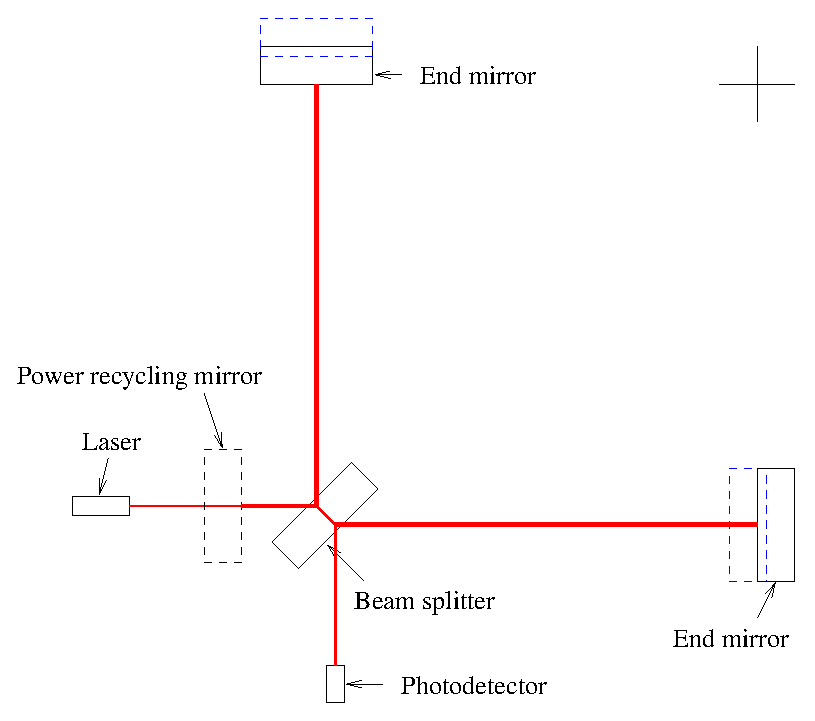
\includegraphics[width=0.5\textwidth]{figs/interferometer}\caption{ A schematic of a
simple Michelson interferometer with power recycling.}\label{interferometer}
\end{center}
\end{figure}

\subsubsection{Interaction of \gws with detectors}
The principle of detecting \gws is based on how they interact with freely falling objects. It
was shown in equations~\ref{gwmotionx} and \ref{gwmotiony} and figure~\ref{ringofparticles} how
particles will react to a passing wave, so we will consider two free masses (our interferometer's
mirrors) placed perpendicular to the direction of propagation of the wave aligned in its $x-y$
plane. If the interferometer beam splitter is placed at a distance $L_0$ from each mirror, then from
equations~\ref{gwmotionx} and \ref{gwmotiony} a \gw will produce a time varying displacement
$\delta{}L$ of the mirrors, for each polarisation, of
\begin{equation}
\frac{\delta{}L^x(t)}{L_0} = \frac{1}{2}(h_+ + h_{\times}),
\end{equation}
and
\begin{equation}
\frac{\delta{}L^y(t)}{L_0} = \frac{1}{2}(h_{\times} - h_+).
\end{equation}
It is the ability of an interferometer to measure such changes in its arm length via the
interference pattern produced that makes them useful for measuring gravitational waves. The
amplitudes given above are for an optimally oriented detector, and if the plane is not perpendicular
to that of the wave 
%and the polarisation angle is not along the $x-y$ plane 
then the amplitude will be reduced by a certain factor (called the beam or antenna pattern). It can
be seen that for longer arm lengths a smaller \gw strain will be measurable for the same
displacement, this means that to detect the sort of source strains discussed above interferometric
\gw detectors will need be large (on the km scale). Even so they will be having to sense
displacements of order $10^{-18}$\,m, roughly equivalent to sensing a displacement of order the
diameter of a Gold atom between the Earth and the moon.

Kilometre scale detectors are still much smaller than the wavelength of the \gw frequencies they
are sensitive to $L_0 \ll \lambda \sim 10^3$\,km for $f \sim 100$\,Hz. This means that in the time
that it takes light to travel down the arms of the \ifo only a small fraction of the displacement
will have taken place. To get round this the light needs to be kept in the arms for about the half
period of the wave. This can be achieved by use of a Fabry-Perot cavity or signal recycling mirror,
which can increase the effective path length of the light by $\sim 100$ \cite{Schutz:1999}.

\subsubsection{Sources of noise}
The displacements to be measured are small, so there will be many sources of noise that threaten
to dominate any \gw signal. The dominant source of noise for an \ifo changes with frequency, and
each will be briefly discussed here (see figure~\ref{geonoisesources} for the noise sources in
G\textsc{eo}\,600).
\begin{figure}[!htbp]
\begin{center}
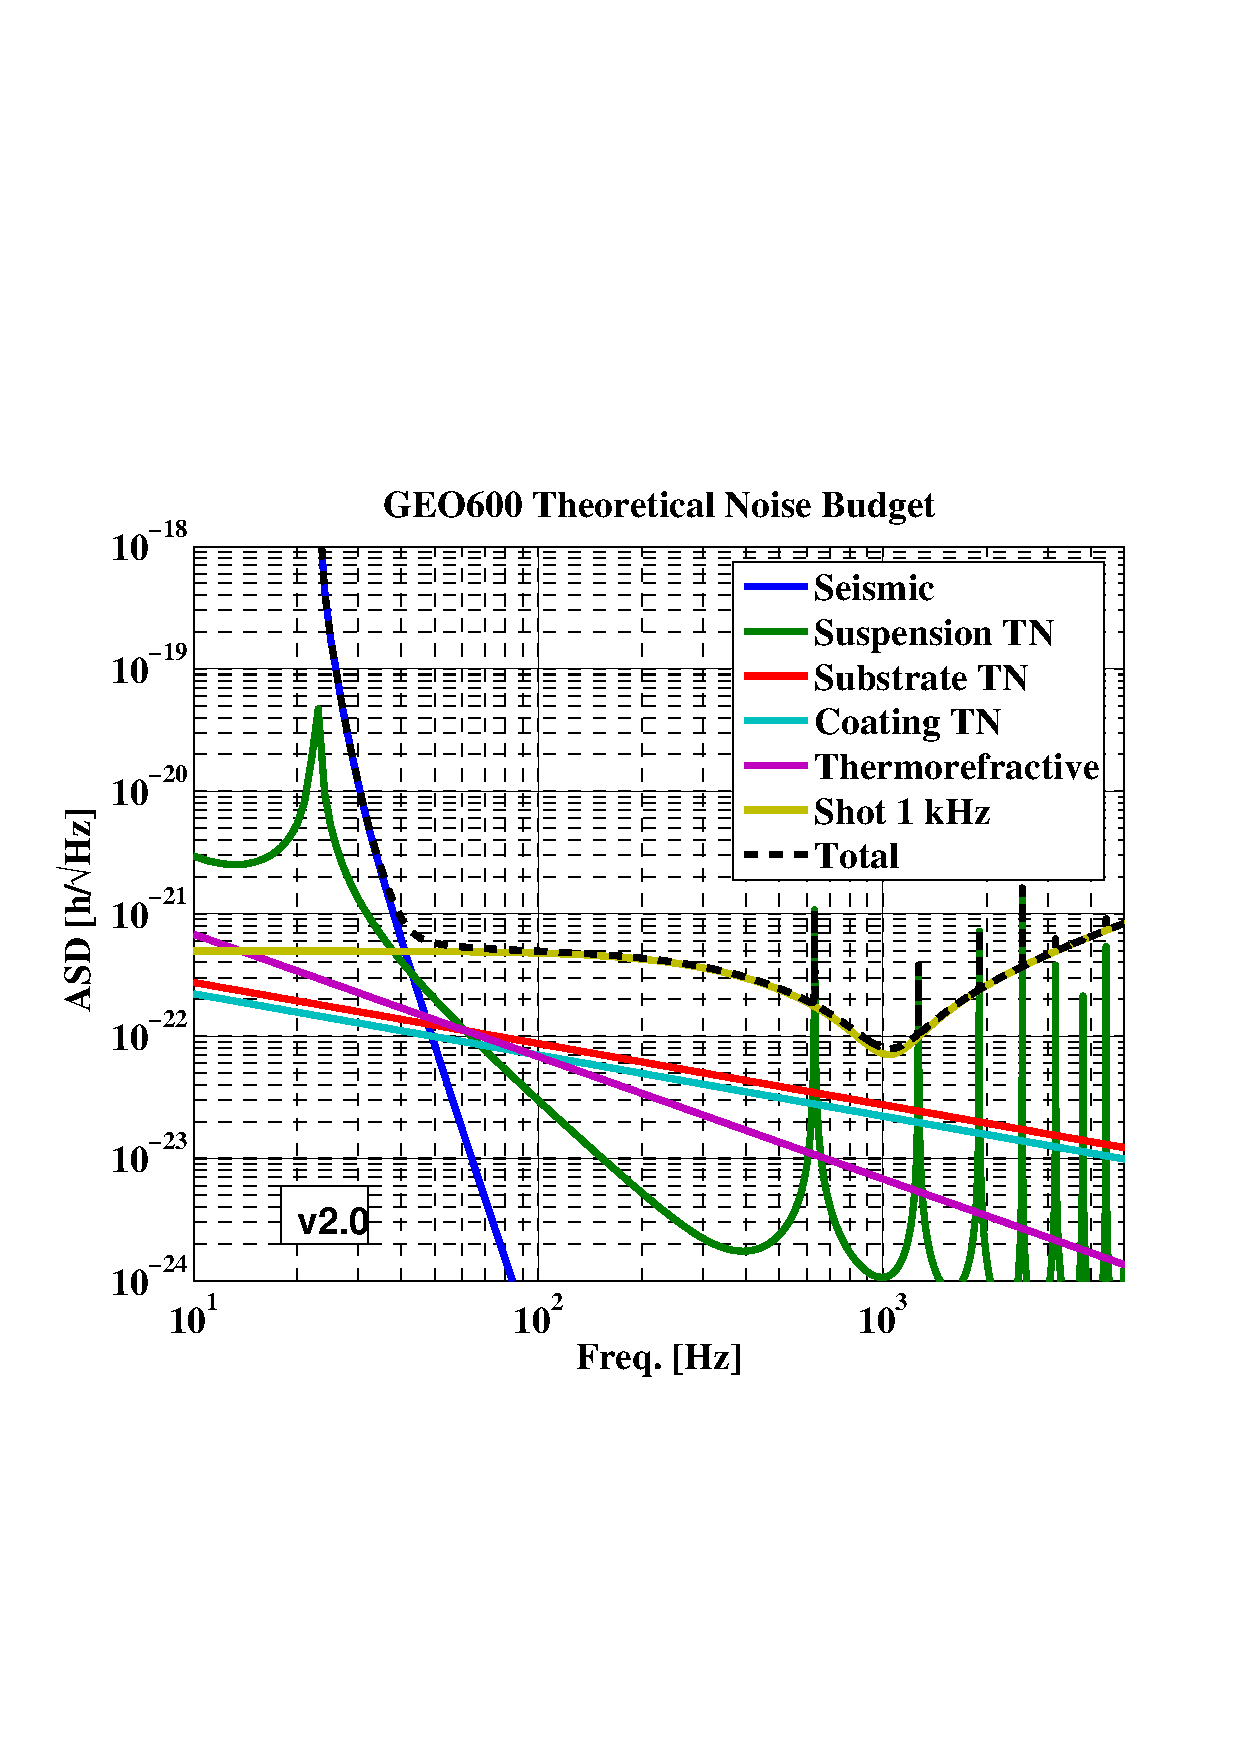
\includegraphics[width=0.5\textwidth]{figs/geo_noise_sources_1000}\caption[Theoretical noise
sources for G\textsc{eo}\,600.]{The theoretical models of the noise sources for G\textsc{eo}\,600
across the sensitive band of the interferometer (taken from
\url{http://www.aei.mpg.de/\~jrsmith/geocurves.html}).}\label{geonoisesources}
\end{center}
\end{figure}

At low frequencies ($<$ few Hz) the underlying noise limit for any ground-based detector will be
gravity gradient noise. This will come from changes in the local gravitational field, from
environmental and possibly man-made sources. The spectrum for this source of noise is inversely
proportional to frequency to a high power and is well below other sources of noise for current
detectors \cite{Schutz:1999}. It could however form a noise wall at low frequencies for future
ground-based detectors. For these low frequencies the only way to get around gravity gradient noise
is to go into space (e.g. LISA \url{http://lisa.jpl.nasa.gov}).

The main low frequency ($\lesssim 30\,$Hz) noise source above gravity gradient noise is seismic
noise. To isolate the mirrors from vibrations they are suspended as pendulums. This provides good
isolation for frequencies above the resonant frequency of the pendulum. Even more effective
isolation can be achieved by stacking several levels of pendulums.

In the mid-range of frequencies ($\sim$100\,Hz-1\,kHz) thermal noise of the masses, mirror coatings
and suspensions will dominate. These components are chosen to have natural frequencies of vibration
outside the main operating frequency range of the detectors, with the suspensions at a few Hz and
masses at several kHz. By choosing materials for these elements with a high quality factor $Q$, like
silica, most of the vibrational energy will be kept to a small frequency range about the natural
frequency. The use of high $Q$ materials means that the interferometers can be operated at room
temperature, but cooling the detectors is being studied as a possible way of reducing thermal noise
in the future.

At high frequencies ($\gtrsim 1$\,kHz) quantum shot noise is the dominant noise source. The fact
that the laser light is made up of quantised photons gives rise to random fluctuations in the number
of photons $N$ at the output. This is a Poisson process so the number of photons will vary as
$\sqrt{N}$, therefore the fractional error on the fluctuations in the number of photons detected
will be reduced by increasing the laser power i.e. increasing $N$. To get the shot noise down to the
low levels needed requires laser powers far higher than any commercially produced lasers reach, so a
technique called power recycling must be used. If the interferometer output is kept on a dark
fringe, so no power is lost at the output, then the only way for power to escape is through the
input, so by placing a mirror in front of the laser this light can be sent back into the cavity
(see figure~\ref{interferometer}). As the mirror optics are high quality little power is lost in
transmission and the power in the cavity is built up. This means that a 10\,W laser is able to give
powers of up to several kW in the cavity. The higher power can however lead to radiation
pressure noise and thermal heating of the mirror and as such a trade off needs to be made.

All these noise sources combine to mean that current interferometers are most sensitive in the
regions of $\sim 10 - 1000$\,Hz, although all sides of the noise curve can be pushed outwards by
applying novel techniques.

\subsubsection{Current detectors}
This thesis will focus on results from the \geo and LIGO detectors. \geo is a joint British/German
600\,m long folded arm Michelson interferometer based near Hannover, with power and signal
recycling\footnote{This is a way of holding light in the cavities for longer at certain frequencies
to enhance the sensitivity in a tunable narrow band, and is achieved by introducing another movable
mirror at the output to put light back into the cavity.} \cite{Willke:2002}. The Laser
Interferometric Gravitational Wave Observatory (LIGO) project \cite{Abramovici:1992} is a US-based
set of three Fabry-Perot cavity interferometers: two collocated in Hanford, WA with 4\,km and 2\,km
arm lengths (called H1 and H2 respectively); and one in Livingston, LA (L1), with a 4\,km arm
length. These detectors make up those used by the LIGO Scientific Collaboration (LSC). All were
under construction and commissioning until they performed their first science run in autumn 2002
(see Abbott {\it et al.}, 2004c \cite{Abbott3:2004}), since when there have been three more science
run periods between which commissioning has taken place. The relative design sensitivities of these
can be seen in figure~\ref{designcurves1year}. Due to its smaller size \geo has been a test bed for
more advanced technologies than LIGO, like monolithic double suspensions and signal recycling, which
will be used in future upgrades to the LIGO instruments i.e. Advanced LIGO.

These detectors are not the only interferometers currently operating. The first large scale \ifo
to successfully make measurements was in fact the Japanese 300\,m-arm-length T\textsc{ama}\,300
detector. This has since performed several data taking runs. The other main \ifo is the
French/Italian 3\,km VIRGO detector near Pisa. VIRGO has been designed with a very elaborate
suspension system to minimise low frequency noise, giving it an advantage over LIGO and \geo below
$\sim 50$\,Hz. VIRGO is still under its commissioning, but should soon join the network of
detectors. 

Along with the interferometers there are several groups with bar detectors. These include AURIGA,
ALLEGRO, EXPLORER and NAUTILUS which have been very active for many years.

\subsubsection{Future detectors}
For ground-based interferometers plans are very advanced for the upgrade and construction of the
next generation. These include the planned upgrade to the current LIGO detectors, by porting some
technologies over from \textsc{Geo}\,600. These should help lower the noise floor by an order of
magnitude (see figure~\ref{designcurves1year}) and expand the volume of space covered by about a
factor of $\sim 1000$. The Japanese have plans for a new detector possibly using cryogenic
technologies to reduce thermal noise. Any upgrades to \geo could see it being focused on the high
frequency region using advanced optical techniques to get below the standard quantum noise limits in
this region.

One of the most exciting future detectors is the space-based detector, the Laser Interferometer 
Space Antenna (LISA). This joint ESA/NASA venture aims to put an \ifo consisting of three
spacecraft forming an equilateral triangle of side 5 million km into space. This would be free
from gravity gradient noise and have a sensitivity over the frequency range of $\sim 0.1-100$\,mHz.
The range of sources in this frequency band should guarantee \gw detection.  

%\subsection{Other methods of detection}
% mention a bit about pulsar timing for v low frequency detection, cmbr polarisation for background
% detection, spacecraft doppler tracking etc.

\section{Current searches}
% say a brief bit about what searches are currently underway
As stated above the LSC interferometers have performed several periods of data taking under science
mode, these have been: S1 from $23^{\rm rd}$ August - $9^{\rm th}$ September 2002 with both \geo
and the LIGO instruments; S2 from $14^{\rm th}$ February - $14^{\rm th}$ April 2003 with just the
LIGO instruments; S3 from $31^{\rm st}$ October 2003 - $9^{\rm th}$ January 2004 with LIGO and
including \geo for two separate periods; and S4 from $22^{\rm nd}$ February - $23^{\rm rd}$ March
2005 with both \geo and LIGO.  Using data from these runs a variety of searches for a large section
of the above sources has been carried out. Here we will briefly summarise some of these results.

In Abbott {\it et al.} (2004a and 2005a) \cite{Abbott:2004, Abbott:2005} searches for continuous
\gws from known pulsars were performed using data from S1 and S2 setting upper limits on $h$ of
$\sim 10^{-24}$ and ellipticities of $\sim 10^{-5}$ for several pulsars (results from the S3 and S4
runs are presented in this thesis). Abbott {\it et al.} (2005c) \cite{Abbott3:2005} shows an all-sky
search for continuous \gws from unknown neutron stars or other sources in the 200-400\,Hz range
using S2 data, with a best upper limit on $h$ of $\sim 4.4\ee{-23}$. Other such all-sky coherent,
semi-coherent and incoherent searches are being used on S2 and more recent data, including a
targeted search for \gws from the LMXB Sco X1, but these results are as of yet unpublished.

Searches for untriggered burst sources have been performed on LIGO data from S1 and S2 in Abbott
{\it et al.} (2004d and 2005d) \cite{Abbott4:2004, Abbott4:2005}, giving a best upper limit on the
event rate for bursts of between 100-1000\,Hz of less than 0.26 per day in the strain amplitude
range $h_{\rm rss} \sim 10^{-20}-10^{-19}\,{\rm Hz}^{-1/2}$\footnote{$h_{\rm rss} \equiv
\sqrt{\int|h|^2 {\rm d}t}$ is the root-sum-squared amplitude spectral density for bursts}. A
coincidence burst search between LIGO and the T\textsc{ama}\,300 detectors during the period of S2
(Abbott {\it et al.}, 2005e \cite{Abbott5:2005}) has given an upper limit of 0.12 events per day
above a strain of $h_{\rm rss} \sim 1-3\ee{-19}\,{\rm Hz}^{-1/2}$ in the frequency range of
700-2000\,Hz. In Abbott {\it et al.} (2005f) \cite{Abbott6:2005} a search has targeted a GRB and set
an upper limit on the radiation for the specific event GRB030329 using LIGO data. For an event
shorter than 150\,ms and around 250\,Hz this gave a strain amplitude upper limit of $h_{\rm rss}
\simeq 6\ee{-21}\,{\rm Hz}^{-1/2}$. Again burst searches for \gws from more recent runs, including
coincidences with G\textsc{eo}\,600, have yet to be published.

The search for inspiral events has included binary neutron stars inspiral (Abbott {\it et al.},
2004b and 2005g \cite{Abbott2:2004, Abbott7:2005}), binary black holes (Abbott {\it et al.}, 2005h
\cite{Abbott8:2005}) and primordial black holes in the Galactic halo (MACHOs) (Abbott {\it et al.},
2005i \cite{Abbott9:2005}). The binary neutron star search had a maximum range of $\sim 1.5$\,Mpc
with an event rate upper limit of 47 per year per Milky Way equivalent galaxy (MWEG) for neutron
stars in the mass range $1-3\,{\rm M}_{\odot}$. The binary black hole search found no events out to
distances of 1\,Mpc for black hole masses between $3-20\,{\rm M}_{\odot}$, giving an upper limit
rate of 38 per year per MWEG. These results are all at 90\% confidence and have been set using S2
data with more up to date results to be published.

Finally in Abbott {\it et al.} (2004e and 2005b) \cite{Abbott5:2004, Abbott2:2005} upper limits on
the stochastic background have been set using LIGO data from S1 and S3. This has given the
increasingly astrophysically interesting upper limit of $\Omega_{\rm gw} < 8.4\ee{-4}$ in the
frequency band 69-156\,Hz.

All these upper limits are from LSC detectors. There are also interesting upper limits on burst,
continuous wave and stochastic sources from the various bar detector groups. Stochastic upper limits
in much lower frequency ranges are also being set via spacecraft doppler tracking and pulsar timing.
Summarising all would require a large review paper and is out of the scope presented here. In the
future all the various detectors should form a large network, the pooling of data from which will be
used to gain the most information about sources and provide the best results.